\section{Architecture and Implementation}

\subsection{Cold Patching}
\label{sec:coldpatch}


To allow for safe instrumentation using iProbe we need to prepare the target application binary. As described in section.\ref{sec:hotpatch}, to enable hot-patching there must be space allocated in the code segment of the binary to re-write instruction.Existing methodologies overwrite target instructions (eg. the starting instruction of the target instruction with a 
jump). However, this requires several additional steps to allocate memory and ensure sanity of the stack frames. 
\\
\indent To reduce complex binary transoformations, we prepare the binary for run-time instrumentation before execution by using a coldpatch process.The steps of this process are shown in the state diagram shown in figure \ref{fig:state_rep}. 

\begin{figure}[hbt]
  \begin{center}
    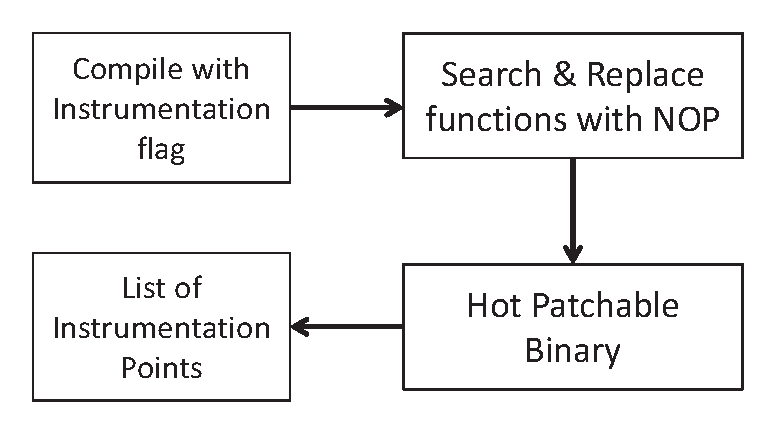
\includegraphics[width=0.45\textwidth]{Images/coldpatch.eps}
    \caption{ColdPatching }
    \label{fig:coldpatch}
  \end{center}
\end{figure}

The first state is an instruction dump of an unmodified normal binary. As can be seen the initial instructions in each function after the call is made to the function are setting up the stack frame and then the main body. Hence, if any of these instructions are overwritten that would lead to potentially illegal execution states. Instead iProbe makes these binaries \textit{``hot-patch ready``} by introduce placeholders in the binary which are used to create empty space. While a compiler transform or flag can be designed based on the target abstraction for instrumentation, for the sake of simplicity we use existing compiler flag options such as ``-finstrument-functions" \cite{gcc_codegen}. As shown in the figure.\ref{fig:state_rep} this flag option generates instrumentation calls at the entry and exit of every function. Just after the entry and before the exit of every function, calls are placed to \emph{\_cyg\_profile\_func\_enter} and \emph{\_cyg\_profile\_func\_exit}. 

As step 2, we use a binary parser performs a linear scan to search and replace each of these function calls with a NOP instruction (state 3). The replacement needs to be done carefully to ensure that there is enough space to overwrite these NOP's with a call to our instrumentation function. Additionally we store the instruction pointer of each of these function calls, the function they belong to, and the symbolic name. By replacing each of these function calls with NOP instructions we introduce a ``zero-probe" effect in the binary, i.e. the modified binary executes the same as the original binary with negligible overhead.
To counter address space layout randomization, we also capture offsets with the starting address of each binary. 
These offsets allow us to use the starting/load address as a anchor to do the instrumentation. In practice we found that the offsets compared to the load address of the executable in binary remain the same, even if load points may be changed.

One of the advantages of preparing and using the cold-patching approach is that natural abstractions in the build process can also be used to choose the scope of instrumentation. Instrumentation scope defines the libraries, files, functions, and modules that can be instrumented. iProbe can be used to pre-define the target files, libraries etc. to be compiled, this can be important in cases where the source code is only partially available to the user. This is common for many large scale projects which use proprietary 3rd party components.


\begin{figure*}[htb]
  \begin{center}
    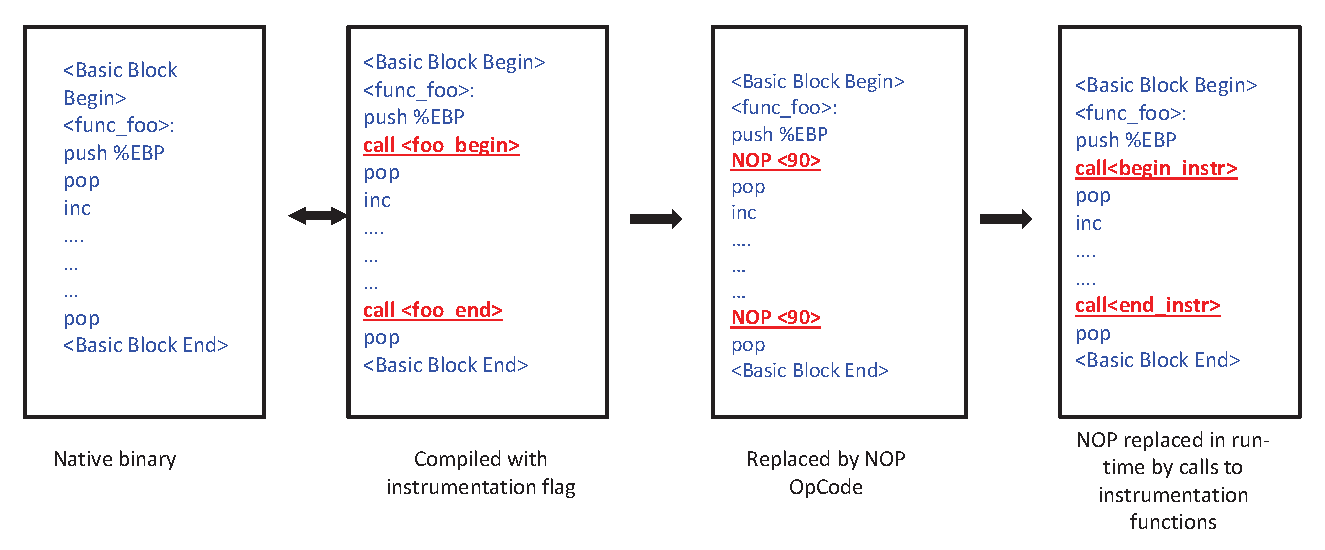
\includegraphics[totalheight=6cm]
    {Images/state-diagram.eps}
    \caption{State Representation for Hot-Patching}
    \label{fig:state_rep}
  \end{center}
\end{figure*}

\subsection{Hot Tracing}
\label{sec:hottracing}



\begin{figure*}[htb]
\begin{center}
  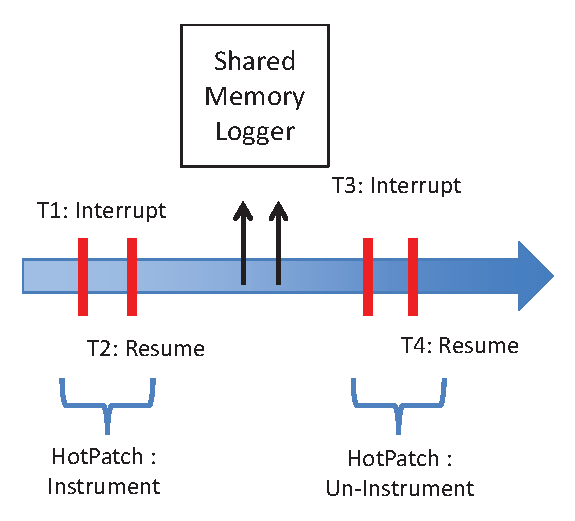
\includegraphics[scale=0.85]{Images/HotTracing.eps}
  \label{fig:hottracing}
  \caption{Hot Tracing Mechanism: 1. Get PID of the target process 2. Instrument and HotPatch the target process 
  3. Shared Memory Logger, and Kernel Tracer 4. Un-Instrument and HotPatch}
\end{center}
\end{figure*}


Once the application is \textit{"hot-patch"} enabled, instrumentation can be applied at run-time. Figure.\ref{fig:hottracing}, shows a step wise diagram of a normal usage case scenario for iProbe. As mentioned earlier in section.\ref{sec:hotpatch} hot-patching needs to load the code segment and activate or deactivate instrumentation as required by the user.Before executing the program all instrumentation code is preloaded in the execution environment. This ensures that the instrumentation library is a part of the code segment of the target application.

The hot-tracer itself is an interactive GUI interface, that assists the user in easy Hot-Tracing. As a first step, the user needs to find the process id of the target process, this can be done by using various utility programs such as ps, ptrace etc. The user then needs to provide the list of instrumentable points which are generated in ColdPatch phase This is the entire list of potential instrumentation points that can be enabled by the user. 

Once provided to the hot-tracer, iProbe then provides the user various function and resource level abstractions to do the instrumentation. The symbolic information used in this step is already read from symbolic information read from the binary at the cold-patching time. The user can choose one or many functions, files or libraries to be the target instrumentation set. This file/component/library to target function relationship\footnotetext[1]{file/component/library to target function relationship may not be available at run-time depending on the amount of debugging information available in the binary, symbolic information may be turned off for production systems} is something which gives a good insight when doing the debugging. 
% **add to the footnote information about binary obfuscation

Function are shown in the following format:
\begin{verbatim}
<Symbol Name, Entry\Exit Point,Source File>
\end{verbatim}

The instrumentation set is taken by the hot-tracer(step 2 in figure.\ref{fig:hottracing}) and the process is instrumented. Our current implementation uses ptrace \cite{ptrace}, a linux utility tool to search and overwrite instrumentation 

\subsection{Dispatcher: Function Selection}

As described in the previous section, once a function is selected for instrumentation a call is made to the instrumentation by hot-patching. However, there can be potentially a large number of functions belonging to the target binary 


\subsection{Implementation}

The current implementation of iProbe has been applied and tested in x86 32 bit and 64 bit systems on an centos 5.0, ubuntu, and red-hat system. Technically, however the implementation can be applied to any existing system by using compiler assistance and hot-patching.
